\documentclass[a4paper]{article}
\usepackage{booktabs}
\usepackage{geometry}
\geometry{
  top=1in,
  inner=1in,
  outer=1in,
  bottom=1in,
  headheight=3ex,
  headsep=2ex
}
\usepackage{amssymb,amsmath}
\usepackage{fontspec}
\usepackage[CJKbookmarks, colorlinks, bookmarksnumbered=true,pdfstartview=FitH,linkcolor=black,citecolor=black]{hyperref}
\usepackage{xeCJK}
\usepackage{xltxtra,xunicode}
\usepackage{listings}
\usepackage{xcolor}
\usepackage{array}

\lstset{basicstyle=\footnotesize\ttfamily,        % size of fonts used for the code
        columns=fullflexible,
        numbers=left,
        numberstyle=\tiny,
        keywordstyle=\color{blue},
        stringstyle=\color[rgb]{0,0.6,0},
        commentstyle=\color[cmyk]{1,0,1,0},
        frame=shadowbox,
        escapeinside=``,
        breaklines=true,
        extendedchars=false,
        xleftmargin=2em,xrightmargin=2em, aboveskip=1em,
        tabsize=4, %tab size
        showspaces=false %no space
       }

\newcommand{\tightlist}{
  \setlength{\itemsep}{0pt}\setlength{\parskip}{0pt}}

% font
\setCJKmainfont[AutoFakeBold]{文泉驿微米黑}
\setmainfont[AutoFakeBold]{Segoe UI}
\setromanfont[AutoFakeBold]{Segoe UI}
\setmonofont[Mapping={}]{Monaco}
\linespread{1.2}\selectfont
\XeTeXlinebreaklocale "zh" 

\begin{document}
\title{\Huge 算法导论课程\\ 第四次上机实验报告}
\author { \vspace{12cm} \\ \LARGE 班级:  1413014  \\ \LARGE 姓名:  乔新文   \\ \LARGE 学号:14130140393} 
\date{ \vspace{4cm} 2017.5.8}

\maketitle
\clearpage

\tableofcontents

\clearpage

\section{综述}

本文档将阐述《算法导论》第四次上机实验代码的详细设计及实现。\\

本次上机实验所用代码均为F\#代码,主要算法和辅助定义均包含在SRAlgorithmLib命名空间下AlgorithmLib4.fs所定义的AlgorithmLib4模块中。\\

算法测试驱动部分在Test.fs中Test模块下的P4函数中,整个程序的入口在Program.fs中。\\

本次实验所有代码均运行在.Net Core上,P1.fsproj为项目配置文件,可在安装有.Net Core的环境中在项目文件夹下使用dotnet run命令运行。\\

\section{题目一}

\subsection{题目}

Bellman-Ford algorithm 

\subsection{实现思路}
Bellman-Ford算法通过对边进行松弛来渐进的降低从源节点到每个节点的最短路径的估计值,并侦测是否存在可以从源节点到达的权重为负值的环路。
\subsection{实现代码}

节点的类型定义\\
其中name记录节点的编号,d记录从源节点到此节点的最短路径权重的上界,π记录其前驱节点
\begin{lstlisting}[language=ML]
    [<Class>]
    type Vertex = 
        val name : int
        val mutable d : float
        val mutable π : Vertex ref option
        new (_name : int, D : float, PI : Vertex ref option) = {name=_name; d=D; π=PI}
\end{lstlisting}

边的类型定义\\
其中u,v记录了边的起始节点和终止节点,weight记录从了边的权重
\begin{lstlisting}[language=ML]
    [<Class>]
    type Edge = 
        val u : Vertex ref
        val v : Vertex ref
        val weight : float
        new (U : Vertex ref, V : Vertex ref, _weight : float) = {u=U; v=V; weight=_weight}
\end{lstlisting}

图的类型定义\\
其中包含边的集合和节点的集合,由邻接矩阵创建并初始化每个节点的d和π
\begin{lstlisting}[language=ML]
    [<Class>]
    type Graphics (adjMatrix : float [,]) as this =
        do
            this.V <- [for i in 0..(Array2D.length1 adjMatrix - 1) -> Vertex(i,infinity,None)]
            this.E <- [
                for i in 0..(Array2D.length1 adjMatrix - 1) do
                    for j in 0..(Array2D.length2 adjMatrix - 1) do
                        if adjMatrix.[i,j] <> infinity || adjMatrix.[i,j] <> 0.0 then
                            yield Edge(ref this.V.[i], ref this.V.[j], adjMatrix.[i,j])
            ]
        [<DefaultValue>] val mutable V : Vertex List
        [<DefaultValue>] val mutable E : Edge List
\end{lstlisting}

初始化操作\\
由于新建图时每个顶点的d和π已被初始化,故这里只设置源节点的d
\begin{lstlisting}[language=ML]
    let InitializeSingleSource (G:Graphics) (s:int) =
        G.V.[s].d <- 0.0
\end{lstlisting}

松弛操作
\begin{lstlisting}[language=ML]
    let Relax (e:Edge)= 
        if (!e.v).d > (!e.u).d + e.weight then
            (!e.v).d <- (!e.u).d + e.weight
            (!e.v).π <- Some(e.v)
\end{lstlisting}

Bellman-Ford算法
\begin{lstlisting}[language=ML]
    let BellmanFord (G:float [,]) (s:int)= 
        let g = Graphics(G)
        InitializeSingleSource g s
        for i = 0 to g.V.Length - 2 do
            List.iter Relax g.E
        not (
                List.exists (fun (item : Edge) -> 
                    (!item.v).d > (!item.u).d + item.weight
                ) g.E
            )
\end{lstlisting}

\subsection{算法测试}

\begin{itemize}
\item
    测试样例:
    \begin{itemize}
    \item
        设置起点为0(无负权回路)\\
       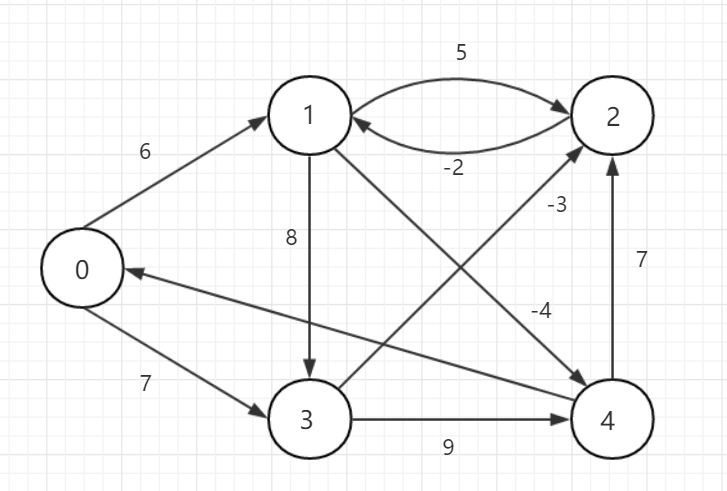
\includegraphics[width=8cm]{4-1-1.png}
    \item
        设置起点为0(存在负权回路)\\
       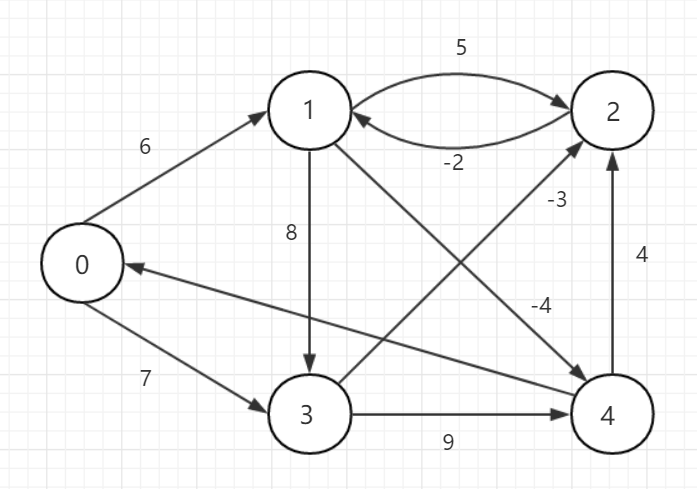
\includegraphics[width=8cm]{4-1-2.png}
    \end{itemize}
\item
    样例输出
    \begin{itemize}
    \item
        true
    \item
        false
    \end{itemize}
\end{itemize}


\section{题目二}

\subsection{题目}

All-pairs shortest path (choose one from the three algorithms)

\subsection{实现思路}

使用动态规划的Floyd算法求解。\\
最短路径的递归求解公式为:
\[c[i,j,k]=
    \left\{
        \begin{array}{ll}
            0 & ,i=j\\
            g[i,j] & ,k=0\\
            min(c[i,j,k-1],c[i,k,k-1]+c[k,j,k-1]) & ,k>0
        \end{array}
    \right.
\]
\subsection{实现代码}

定义邻接链表的节点元素。

\begin{lstlisting}[language=ML]
    [<Struct>]
    type Node = 
            val ID:int
            val Weight:float
            new (id:int,weight:float) = {ID = id; Weight = weight}
\end{lstlisting}

邻接链表到邻接矩阵的转换方法

\begin{lstlisting}[language=ML]
    let AdjListToAdjMatrix (adjList : Set<Node>[]) =
        let adjMatrix = Array2D.create adjList.Length adjList.Length infinity
        for i = 0 to adjList.Length - 1 do
            adjMatrix.[i,i] <- 0.0
            for j in adjList.[i] do
                adjMatrix.[i,j.ID] <- j.Weight
        
        adjMatrix
\end{lstlisting}

计算所有节点对间最短距离的Floyd算法\\
其中,m保存了节点间的最短距离,s保存了节点对间最短路径上的中间节点

\begin{lstlisting}[language=ML]
    let Floyd (G:float [,]) = 
        let n = Array2D.length1 G
        let m = Array2D.copy G
        let s = Array2D.create n n -1
        for i = 0 to n - 1 do
            for j = 0 to n - 1 do
                for k = 1 to n - 1 do
                    let q = m.[i,k] + m.[k,j]
                    if q < m.[i,j] then
                         m.[i,j] <- q
                         s.[i,j] <- k
        (m,s)
\end{lstlisting}

递归的打印最短路径

\begin{lstlisting}[language=ML]
    let rec PrintFloyd (s:int [,]) (i:int) (j:int) = 
        if i = j then
            printf "%A " i
        elif s.[i,j] = -1 then
            printf "%A %A " i j
        else
            PrintFloyd s i s.[i,j]
            PrintFloyd s s.[i,j] j
\end{lstlisting}

\subsection{算法测试}

\begin{itemize}
\item
    测试样例:图结构
    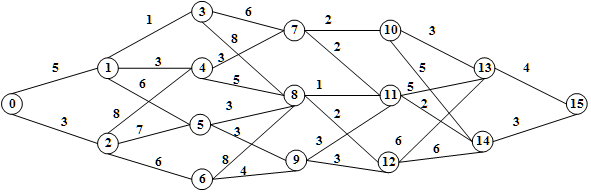
\includegraphics[width=12cm]{4-2.png}
    为节约篇幅,此处仅给出4组随机挑选的起点终点对
    \begin{itemize}
    \item
        起点0,终点15
    \item
        起点0,终点8
    \item
        起点6,终点10
    \item
        起点3,终点15
    \end{itemize}
\item
    样例输出(每对起点终点间的最短路径):
    \begin{itemize}
    \item
        0 1 1 4 4 7 7 11 11 14 14 15
    \item
        0 1 1 4 4 8
    \item
        6 8 8 4 4 7 7 10
    \item
        3 7 7 11 11 14 14 15
    \end{itemize}
\end{itemize}

\section{题目三}

\subsection{题目}

8-queen problem (back backing)

\subsection{实现思路}

由于8皇后问题是n皇后问题的一个特例,故直接求解n皇后问题。\\
设置棋盘为n*n的方形棋盘,棋盘行和列均为0——(n-1)。\\
使用一个长度为n的一维数组s用于存放结果,即s.[i]表示第i行的皇后应放的列。\\
回溯判断在while循环的第一行,若当前行的棋子是否在棋盘外,则当前行复位,回溯到上一行。\\
合法摆法的判断条件是最后一行的棋子位置是否合法,若合法,则为一个有效的摆法。
\subsection{实现代码}

判断当前行放置的皇后是否合法,不合法的条件是当前行皇后和其他已放置的皇后在同一列 \[s.[i] = s.[n]\] 或在同一斜线 \[abs (n - i) = abs(s.[n] - s.[i])\]

\begin{lstlisting}[language=ML]
    let canPlace (s: int []) (n:int) =
        let mutable i = 0
        let mutable result = true
        while result && i < n do
            if s.[i] = s.[n] || abs (n - i) = abs(s.[n] - s.[i]) then
                result <- false
            else
                i <- i + 1
        result
\end{lstlisting}

初始化结果数组并开始回溯算法。

\begin{lstlisting}[language=ML]
    let nQuene n =
        let s = Array.create n 0
        let mutable k = 0
        while s.[0] < n do
            if s.[k] >= n then
                s.[k] <- 0
                k <- k - 1
                s.[k] <- s.[k] + 1
            else
                if canPlace s k then
                    if k = n - 1 then
                        printfn "%A" s
                        s.[k] <- s.[k] + 1
                    else 
                        k <- k + 1
                else
                    s.[k] <- s.[k] + 1
\end{lstlisting}

\subsection{算法测试}

\begin{itemize}
\item
    测试样例:
    \begin{itemize}
    \item
        4皇后
    \item
        8皇后
    \end{itemize}
\item
    样例输出
    \begin{itemize}
    \item
        4皇后可行解:\\
        \ [1; 3; 0; 2]\\
        \ [2; 0; 3; 1]
    \item
        8皇后解法:\\
        8皇后问题有92钟可行解,由于篇幅所限,故此处仅列出前4个可行解:\\
        \ [0; 4; 7; 5; 2; 6; 1; 3] \\
        \ [0; 5; 7; 2; 6; 3; 1; 4] \\
        \ [0; 6; 3; 5; 7; 1; 4; 2] \\
        \ [0; 6; 4; 7; 1; 3; 5; 2]

    \end{itemize}
\end{itemize}

\section{题目四}

\subsection{题目}

0-1 knapsack problem (back tracking)

\subsection{实现思路}

如果不涉及剪枝操作的话,回溯算法等价于一个左子树优先展开的深度优先遍历过程。\\
回溯算法求解01背包问题可转化为在所有合法的选择可能下选择总价值最大的过程。\\
合法条件是总重量小于等于背包容量。

\subsection{实现代码}

while循环用于控制整个深度遍历过程,其终止条件为根元素越界,由于深度优先遍历中是子节点先于父节点遍历完成,故当根节点越界时,整棵树也已经遍历完成。

\begin{lstlisting}[language=ML]
    let knapsack01 v (w:float []) s =
        let result = Array.create (Array.length v) 0
        let mutable maxSum = 0.0
        let mutable k = 0
        while result.[0] < 2 do
            if result.[k] >= 2 then
                result.[k] <- 0
                k <- k - 1
                result.[k] <- result.[k] + 1
            else
                if k >= result.Length - 1 then
                    if s >= Array.sum (Array.map2 (fun item1 item2 -> (float item1) * item2 ) result w) then
                        let sum = Array.sum (Array.map2 (fun item1 item2 -> (float item1) * item2 ) result v)
                        if maxSum < sum then
                            maxSum <- sum
                    result.[k] <- result.[k] + 1
                else
                    k <- k + 1
        maxSum
\end{lstlisting}
下述部分用于树展开到叶子节点,即获得一种选择方案时进行筛选,计算此方案的总重量是否合法并判断是否要更新记录的价值总和上界。
\begin{lstlisting}[language=ML]
                if k >= result.Length - 1 then
                    if s >= Array.sum (Array.map2 (fun item1 item2 -> (float item1) * item2 ) result w) then
                        let sum = Array.sum (Array.map2 (fun item1 item2 -> (float item1) * item2 ) result v)
                        if maxSum < sum then
                            maxSum <- sum
                    result.[k] <- result.[k] + 1
                else
                    k <- k + 1
\end{lstlisting}

\subsection{算法测试}

\begin{itemize}
\item
    测试样例:
    \begin{itemize}
    \item
        背包总空间: 100 \\
        物品重量序列 \ [50;30;45;25;5] \\
        对应的物品价值 \ [200;180;225;200;50]
    \end{itemize}
\item
    样例输出
    \begin{itemize}
    \item
        可容纳的最大价值 \ 605
    \end{itemize}
\end{itemize}

\end{document}
